\section{Discussion}
This section will discuss the findings from the interview study. For problems that were mentioned in the user tests, a possible solution will be discussed. For motivational factors, ways to further improve these factors will be taken into consideration.

\subsection{Hindering factors: missing interface components}
In this subsection, problems that can be solved with additional interface components will be discussed.

\subsubsection*{Overview of currently set filters}
Multiple participants had trouble recognizing what data filters were applied for the current visualization. The idea that the filters can be changed on top of the notebook and will then influence the rest of the visualization does not seem to work, especially on smaller laptops, as this resulted in a lot of scrolling.

\begin{figure}[htbp]
    \fbox{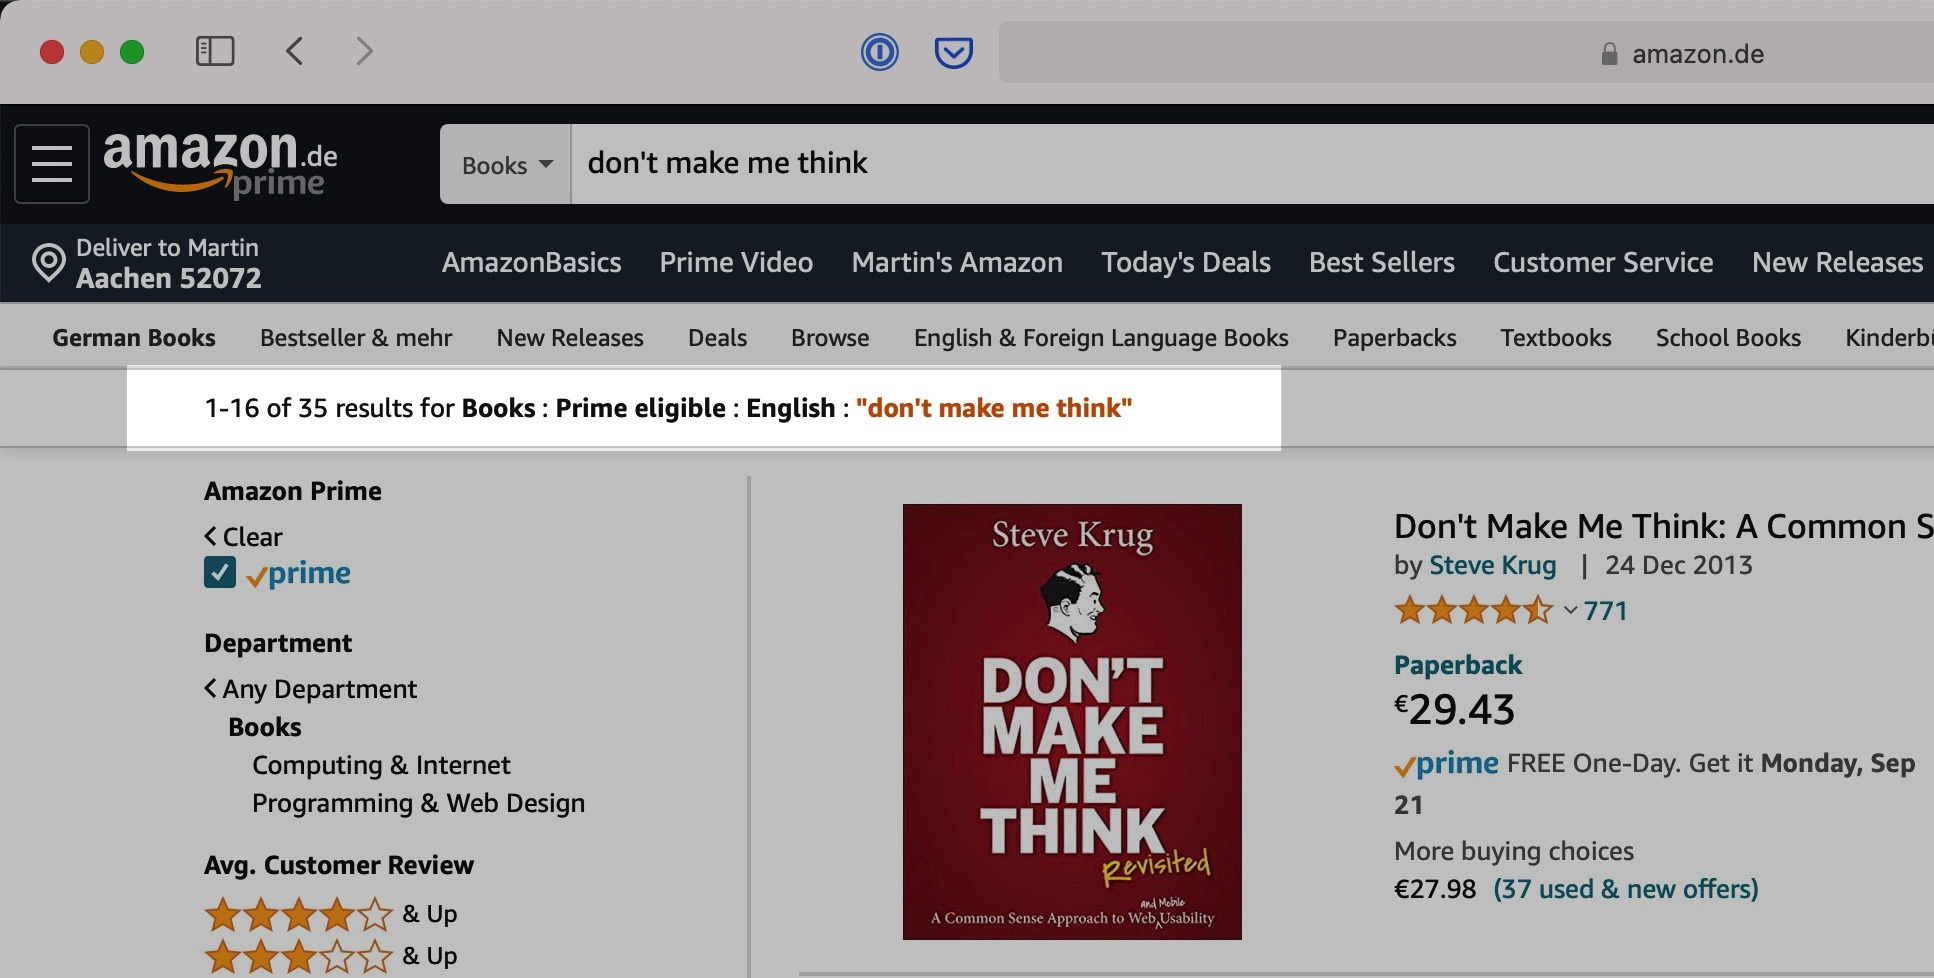
\includegraphics[width=\linewidth]{images/amazon_filters.jpg}}
    \caption{The Amazon search is filtered to English-language books which are eligible to prime-shipping, with the search input \emph{don't make me think}}
    \label{fig:amazon_filters}
\end{figure}

This means that the filter status should be visible directly next to the visualization. This way, participants would not need to search for the current filter status. Rather, the status would almost always be in view while interpreting the visualizations. There are two possible ways to show the filters near the visualizations:
\begin{enumerate}
    \item \textbf{Show a descriptive text above the visualization:} using a text to show the status of the filter could help participants to quickly understand what kind of data the visualization is showing at the moment. One example of this technique can be found on Amazon, as seen in figure \ref{fig:amazon_filters}. This technique is especially useful when a lot of different filters can be applied.
    \item \textbf{Show the filter toggles right next to the visualization:} instead of showing the filter status as a text, showing them with the actual toggles would allow users to change the filters right next to the visualization.
\end{enumerate}

\begin{figure}[h!tbp]
    \fbox{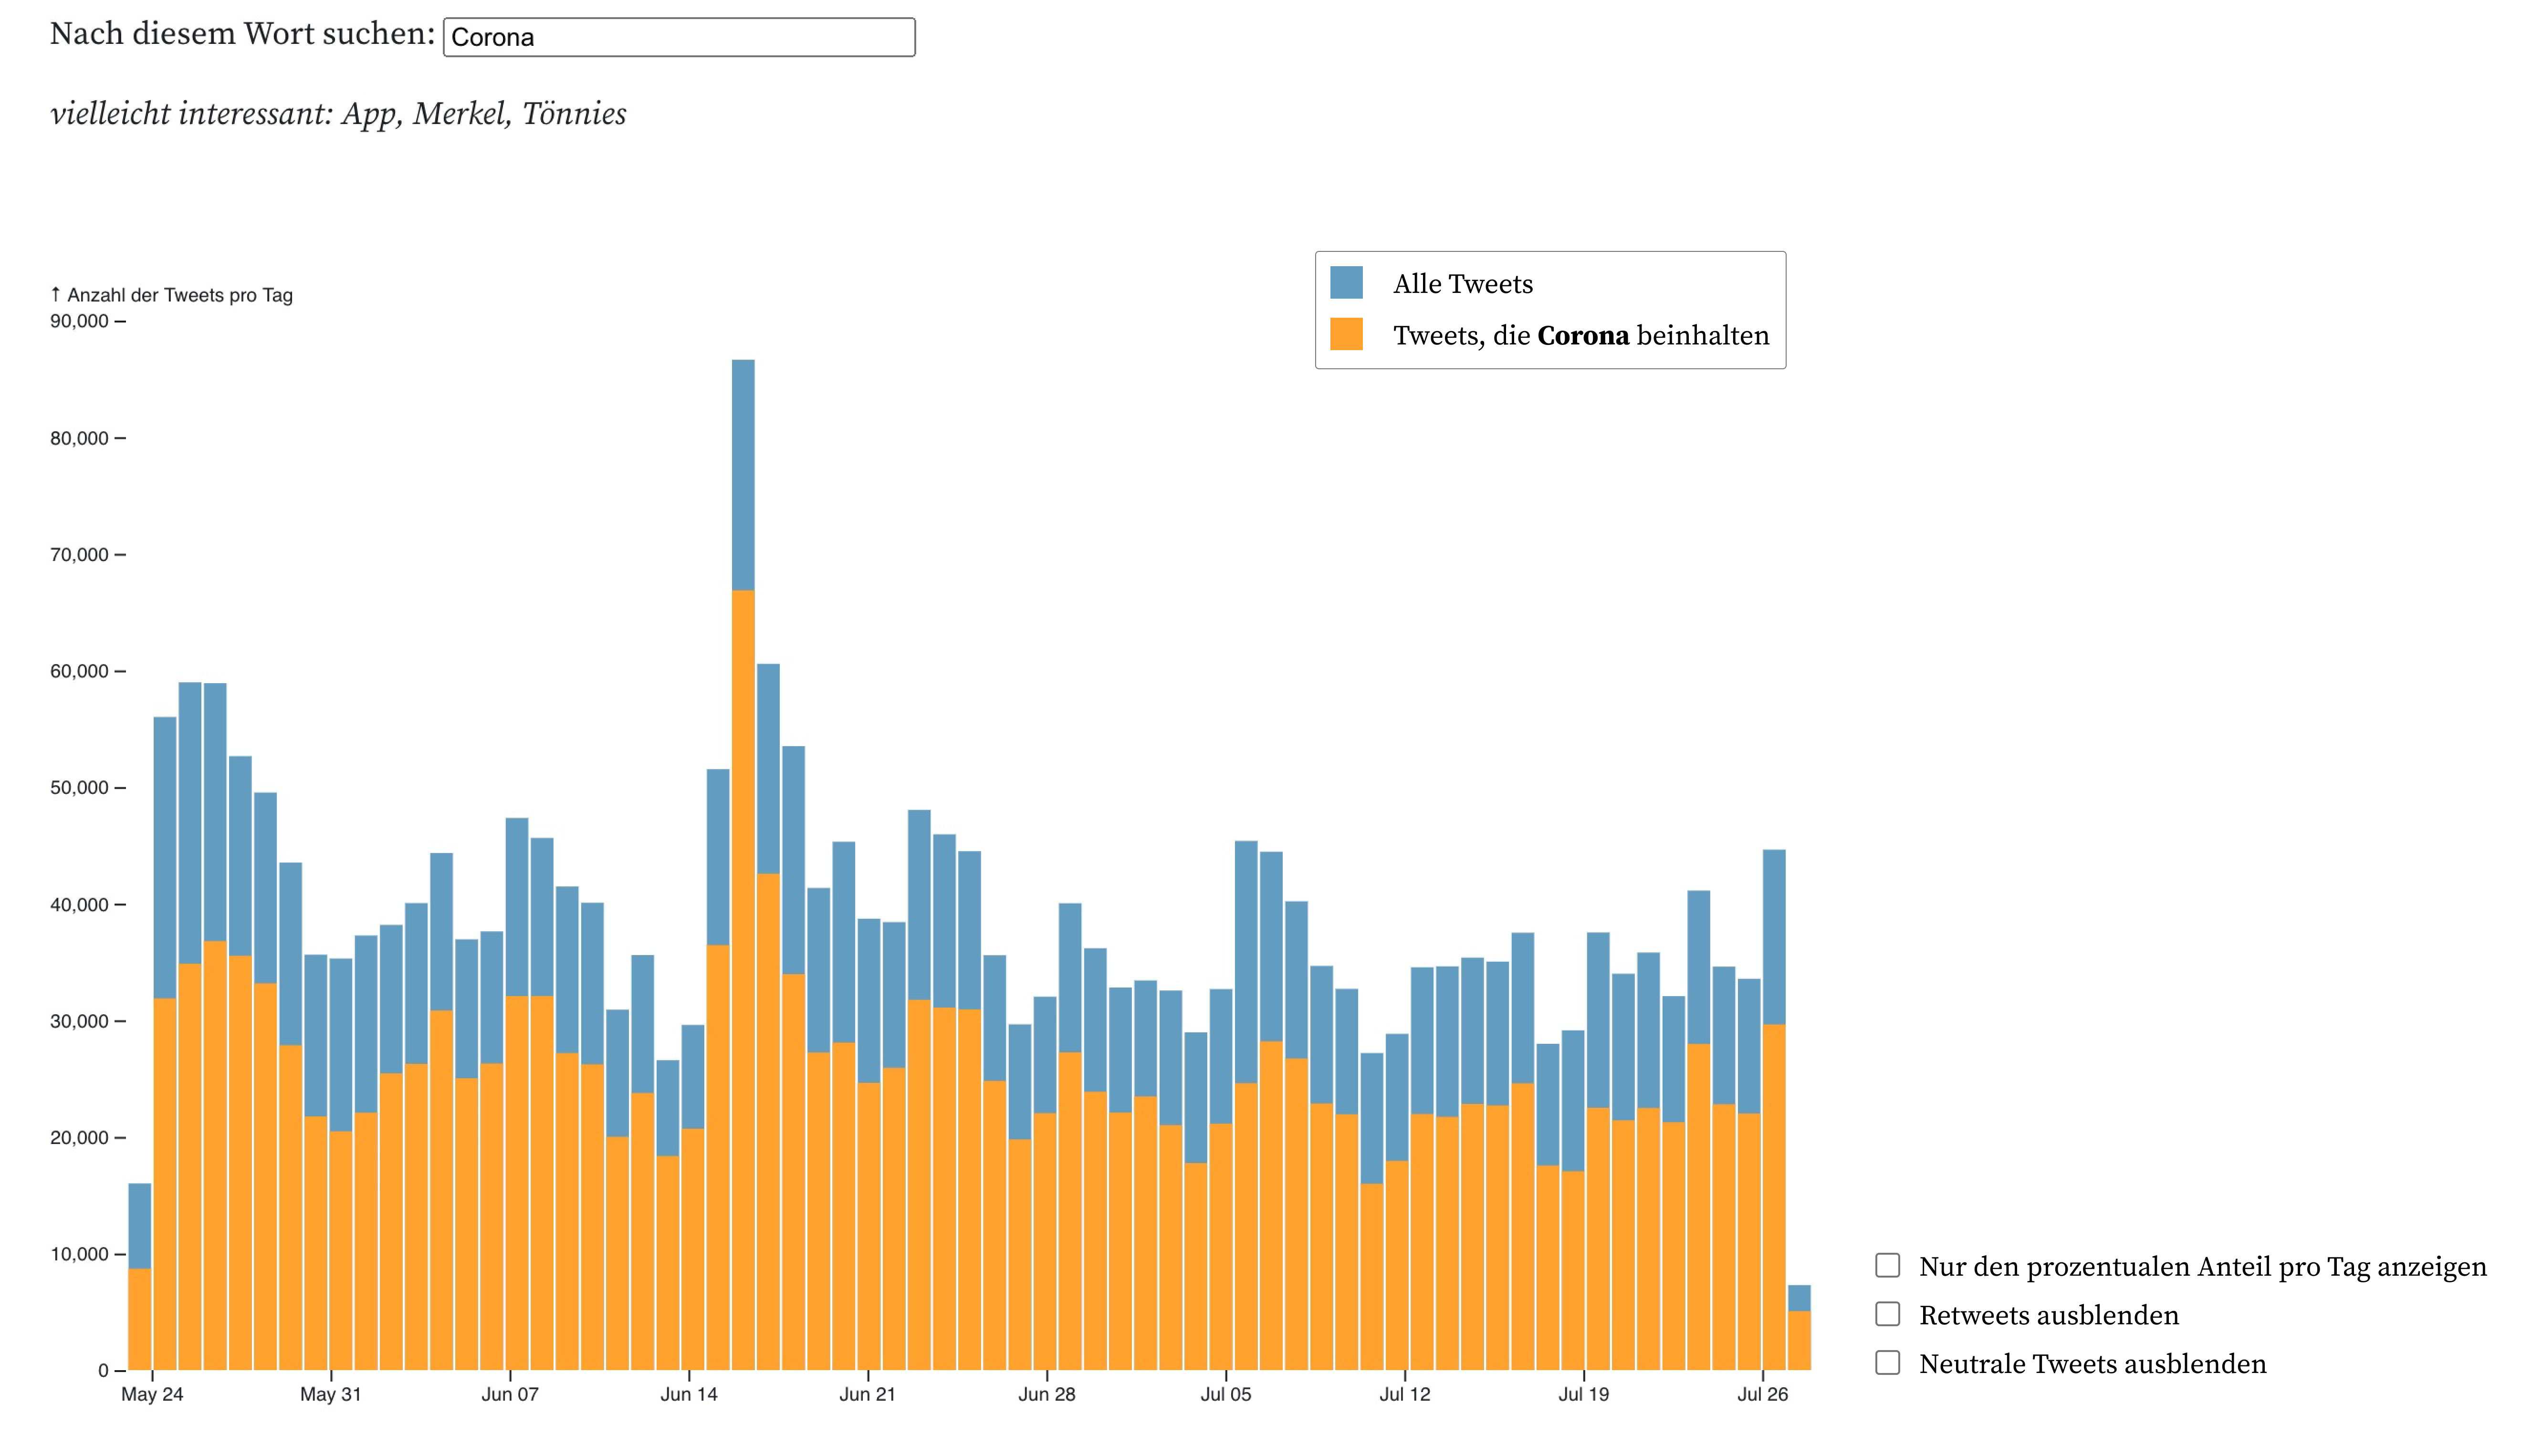
\includegraphics[width=\linewidth]{images/legend_and_filters.png}}
    \caption{Proposed layout of the tweet volume with a legend and filters directly next to the graph}
    \label{fig:legend_and_filters}
\end{figure}

Showing the filter toggles right next to the visualizations seems like a straightforward idea. However, this raises the question if the filters of the two visualizations should be linked or not, i.e., should the filter of the sentiment graph change as well when the filter of the volume graph is changed or not. To decide this, further studies should be conducted to see if the synchronicity of the data visualizations is helpful or not. This study did not examine if it helps users to have a single filter context with several visualizations or not. During the exploration phase in the interview, however, the participants did not seem to switch a lot between the tweet volume and the sentiment chart. This could suggest that having a single filter applied to both visualizations is not a necessity. In this case, using two filter sets that are independant from each other could avoid user confusion as only explicit user actions have an influence on the visualzation.

\subsubsection*{Color legend}
Another missing interface component are colored legends. During user testing, several problems arose because of the missing legend. For one, the graph was less self-contained. Users were forced to read the explanatory texts that accompanied the graph to be able to understand what the different colors mean. Another problem with the textual explanation of colors was that different participants would have named the colors differently than the text did. A legend like the one shown in figure \ref{fig:legend_example} could have helped identifying the colors more easily, as well as making the graph more self-explanatory.

Figure \ref{fig:legend_and_filters} shows a proposed addition to the tweet volume-graph. Implementing these changes makes the current filter status more obvious and lets users toggle the different filters without needing to scroll to the top of the notebook again. The legend with dynamic labelling, which includes the search term the user entered, makes the graph more self-contained.

The added legend could also help solve the layout problem that participants mentioned. With the explanatory texts no longer neccessary to understand the graphs, the texts serve as additional explanation and, as such, can remain below the graph itself.

\subsubsection*{Loading indicator}
Another component that was missing from the interface was an indicator that new data was fetched from the server. One possibility to show this fetching would be to show a small loading indicator next to the word filter. This, however, could be not visible enough. Another possiblity would be to show in the visualizations themselves that new data is being fetched. As fetching takes about 5 seconds and the visualzations have not been updated before the fetching is complete, it should not be a big problem to visually hide the visualizations during the fetching stage. A possible solution for this can be seen in figure \ref{fig:fetching_state}.

\begin{figure}[htbp]
    \fbox{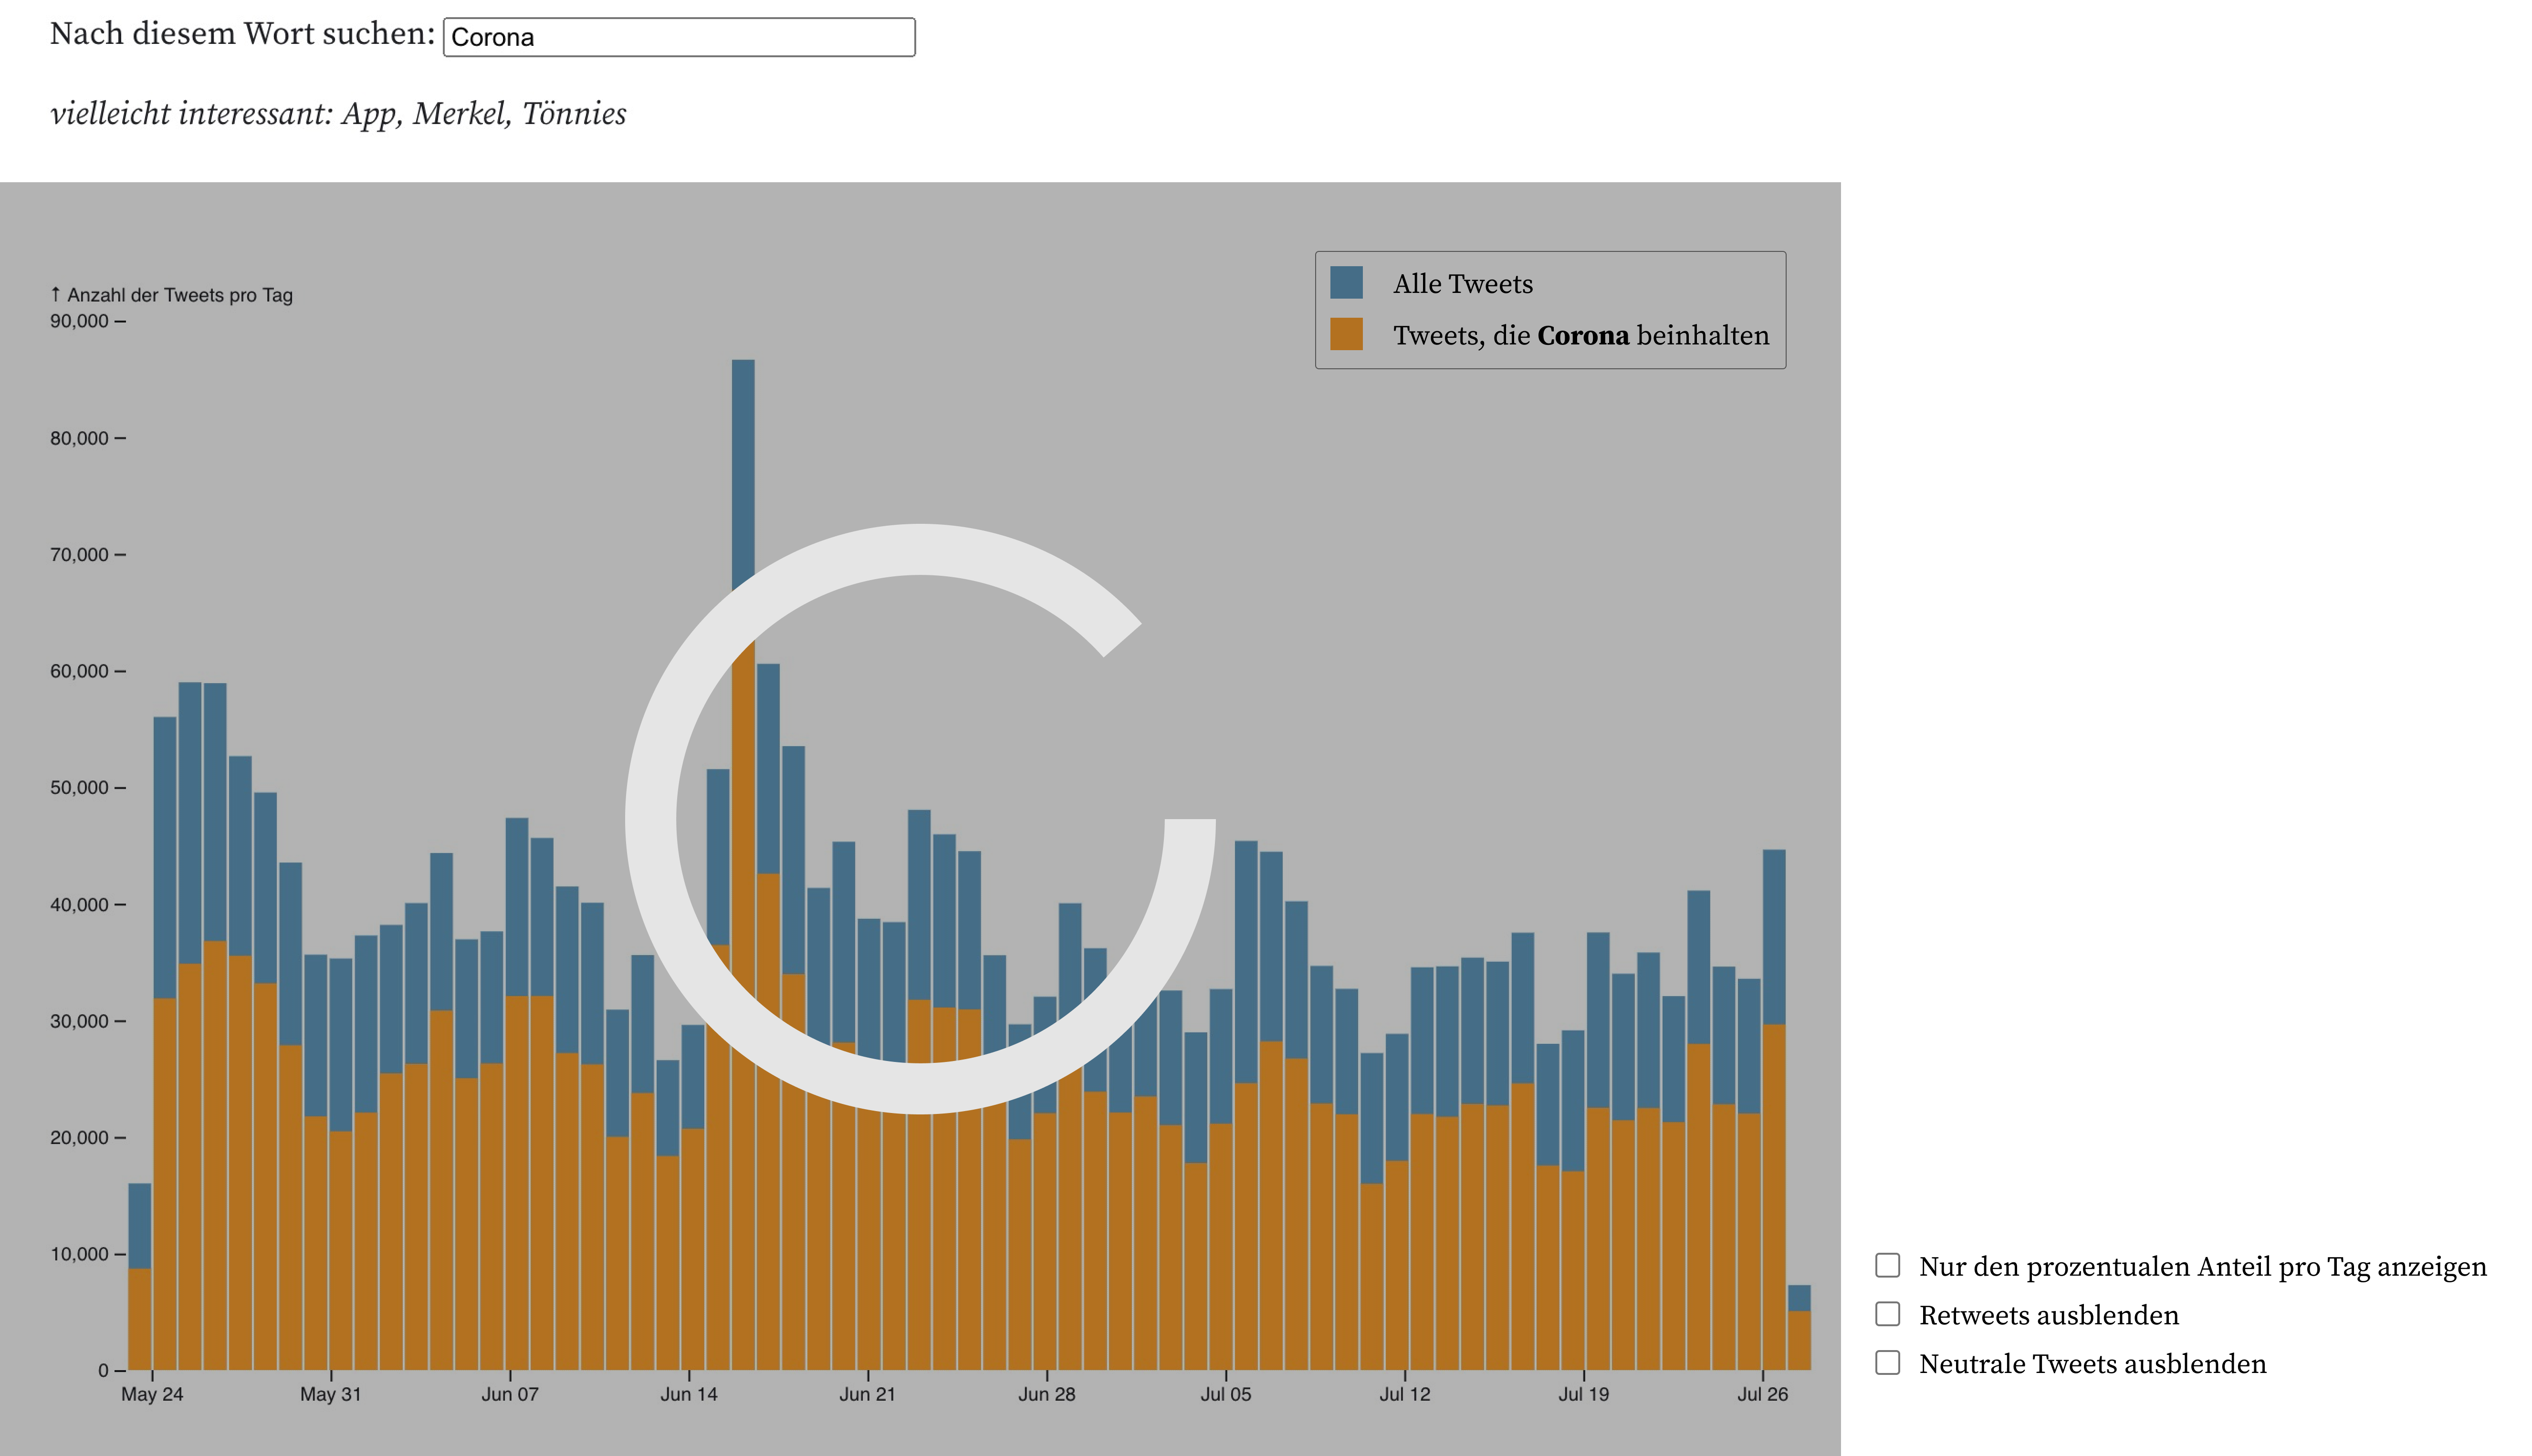
\includegraphics[width=\linewidth]{images/fetching_state.png}}
    \caption{Proposed solution to show that new data is being retrieved from the server}
    \label{fig:fetching_state}
\end{figure}

\subsubsection*{Tooltips for the sentiment graph}
During the user tests, the participant expected to find tooltips for both graphs once they found the tooltip in the volume graph. This means that tooltips should either be used globally for all visualizations---at least where the additional information provided by the tooltip adds to the value---or not at all. As the tooltip in the volume graph helped participants to further explore 

\subsection{Technical limitations}
This section discusses findings from the interview where technical limitations hindered participants from solving tasks. Some of these limitations were conscious trade-offs for this prototype version. Nonetheless, these issues should be adressed if a tool based on this prototype should be further developed.

\subsubsection*{Fixed data set}
The fixed data set came up in one interview where the participant tried to scroll the data set to reveal even more days. This revealed one of the bigger disadvantages of using Twitter's streaming API to collect tweets in real time (see chapter \ref{sec:fetchedData}). Using this method guarantees the most complete data set on the free tier of Twitter's API, at least from the time the data collection is started. The downside is that using this API makes it impossible to access past tweets. Users of the tool thus have to recognize a potentially interesting topic very early, start the data collection, and then wait some time until enough data has been gathered.

Using the paid API to access Twitter's archives could solve this problem, at least in parts. The paid access to Twitter's archives allows to scan the past 30 days of activity on Twitter, which could give a 'headstart' to the data collection. For a final version of this tool, a split approach could be possible: use the real-time data collection of a specific topic using the streaming API, and simultaneously fetch the last 30 days of Twitter activity to this topic. This would mean that users would get direct access to the past month of tweets directly from the beginning of the data collection, elminimating the need to wait some days before they can gather meaningful results from Twitter.

\subsubsection*{Word filter instead of fuzzy search}
Another problem that nees further technical work is how the word filter operates. The current implementation acts as a case-insensitive filter which looks for parts of words. This means that, if a user enters \emph{App}, tweets containing these sorts of texts will be found:

\begin{itemize}
    \item I like this \textbf{App} a lot
    \item Whats\textbf{App} collects your data
    \item What kind of video \textbf{app} would you recommend?
    \item I'm not angry, just dis\textbf{app}ointed
\end{itemize}

This is different from how a search engine, like DuckDuckGo or Google, works. These engines use a so-called \emph{fuzzy search} which not only looks for the word itself, but also catches typos, looks for synonyms, and so on.

Using a fuzzy search would allow users to explore the database more efficiently. During testing, for example, typos would mean that little to no results were found. The participant, however, thought that there was not a lot of Twitter activity about the specific topic. After she was told to correct the typo, she noticed an interesting pattern in the tweet activity and was able to interpet the data further. This means that it could be helpful to implement fuzzy search if the prototype should be further developed.

